\section{Struttura lessicale di \SBF}

\subsection*{Parole riservate}
Le parole riservate in \SBF\ sono le seguenti:
\begin{gather*}
\If,\ \Else,\ \Do,\ \While,\ \Def,\ \Return,\ \Var,\ \texttt{Array},\ \False,\ \True,\ \texttt{until},\ \texttt{by},\\
 \texttt{Null},\ \texttt{Char},\ \texttt{String},\ \texttt{Int},\ \texttt{Float},\ \texttt{Bool},\ \texttt{val},\ \texttt{ref},\ \texttt{res},\ \texttt{valres}.
\end{gather*}

\subsection*{Identificatori}

Un identificatore $\token{Ident}$ è una lettera o il carattere '\_' seguiti da una sequenza arbitraria di lettere, cifre e del carattere '\_'.

\subsection*{Letterali}
Vi sono letterali per numeri interi, numeri in virgola mobile, singoli caratteri, booleani, stringhe. Essi seguono le convenzioni della maggior parte dei linguaggi di programmazione.
\begin{align*}
\token{Literal} ::=\ 
& \token{Int}\\
|\ & \token{Float}\\
|\ & \token{Char}\\
|\ & \token{Bool}\\
|\ & \token{String}\\
|\ & \texttt{Null}
\end{align*}

\subsection*{Commenti}
I commenti in \SBF\ sono di due tipi:
\begin{itemize}
	\item i commenti di una riga sono sequenze di caratteri che iniziano con \verb$//$ e finiscono al termine della riga;
	\item i commenti multi-riga sono sequenze di caratteri che iniziano con \verb$/*$ e terminano con \verb$*/$. Non possono essere annidati.
\end{itemize}

\subsection*{Caratteri di spaziatura}
I token possono essere separati dai caratteri di spaziatura standard o commenti.

\section{Struttura sintattica di \SBF}
\begin{itemize}
	\item Un \emph{programma} è una sequenza di dichiarazioni.
	
	\item Una \emph{dichiarazione} ha una delle seguenti forme:
	\begin{itemize}
		\item \emph{Dichiarazione di variabili}
		\begin{align*}
		\token{Decl} ::=\ &\texttt{var}\ \token{Ident} \texttt{:}\ \token{TypeSpec}\ \texttt{=}\ \token{Expr}\ \texttt{;}\\
		|\ &\texttt{var}\ \token{Ident} \texttt{:}\ \token{TypeSpec} \texttt{;}
		\end{align*}
		
		\item \emph{Dichiarazione di funzioni e procedure}
		\begin{align*}
		\token{Decl} ::=\ & \texttt{def}\ \token{Ident}\ \token{ParamClauses} \texttt{:}\ \token{TypeSpec}\ \texttt{=}\ \token{Expr}\ \texttt{;}\\
		& \texttt{def}\ \token{Ident}\ \token{ParamClauses} \texttt{:}\ \token{TypeSpec}\ \texttt{=}\ \token{Block}\\
		& \texttt{def}\ \token{Ident}\ \token{ParamClauses}\ \texttt{=}\ \token{Expr}\ \texttt{;}\\
		& \texttt{def}\ \token{Ident}\ \token{ParamClauses}\ \texttt{=}\ \token{Block}
		\end{align*}
		
	\end{itemize}
	dove $\token{TypeSpec}$ è una specifica di tipo, che ha la forma
	\begin{align*}
	\token{TypeSpec} ::=\ &\token{SimpleType}\\
	|\ &\texttt{*}\ \token{TypeSpec}\\
	|\ &\texttt{Array}\ \texttt{[}\ \token{TypeSpec}\ \texttt{]}\ \texttt{(}\ \token{Int}\ \texttt{)}\\
	\token{SimpleType} ::=\ &\texttt{Bool}\ |\ \texttt{Char}\ |\ \texttt{Int}\ |\ \texttt{Float}\ |\ \texttt{String}
	\end{align*}
	mentre l'elemento $\token{ParamClauses}$ è una sequenza, non vuota, di $\token{ParamClause}$, e ciascun $\token{ParamClause}$ ha la forma
	\begin{equation*}
	\token{ParamClause} ::=\ \texttt{(}\ \token{Params}\ \texttt{)}
	\end{equation*}
	$\token{Params}$ è una sequenza, che può essere vuota, di elementi separati da virgola della forma
	\begin{equation*}
	\token{Param} ::=\ \token{Mode}\ \token{Ident}\ \texttt{:}\ \token{TypeSpec}
 	\end{equation*}
 	dove $\token{Mode}$ indica la modalità di passaggio del parametro
 	\begin{equation*}
 	\token{Mode} ::=\ \texttt{val}\ |\ \texttt{ref}\ |\ \texttt{res}\ |\ \texttt{valres}
	\end{equation*}
	
	Ad esempio, una specifica di tipo valida è $\texttt{Array[*Int](2)}$, che indica un array di puntatori ad interi di dimensione $2$. Ad esempio, una definizione di funzione valida è
	\begin{verbatim}
	def foo(val a: Array[*Int](2), val p: *Int)(val x: Int): Int = 
		*a[1] + *a[2] + *p + x;
	\end{verbatim}
	Essa prende come parametri un array di puntatori ad interi, un puntatore ad un intero e un intero e restituisce un intero.
	
	\item Un \emph{blocco} è una sequenza di istruzioni racchiuse fra parentesi graffe.
	\begin{equation*}
	\token{Block} ::=\ \texttt{\{}\ \token{StmtList}\ \texttt{\}}
	\end{equation*}
	
	\item Una \emph{istruzione} ha la forma:
	\begin{align*}
	\token{Stmt} ::=\ &\token{Decl}\\
	|\ &\token{Block}\\
	|\ &\token{LExpr}\ \token{OpAssign}\ \token{Expr}\ \texttt{;}\\
	|\ &\texttt{if}\ \texttt{(}\ \token{Expr}\ \texttt{)}\ \token{Stmt}\\
	|\ &\texttt{if}\ \texttt{(}\ \token{Expr}\ \texttt{)}\ \token{Stmt}\ \texttt{else}\ \token{Stmt}\\
	|\ &\texttt{for}\ \texttt{(}\ \token{Ident}\ \texttt{<-}\ \token{Expr}\ \texttt{until}\ \token{Expr}\ \texttt{by}\ \token{Expr}\ \texttt{)}\ \token{Stmt}\\
	|\ &\texttt{do}\ \token{Stmt}\ \texttt{while}\ \texttt{(}\ \token{Expr}\ \texttt{)}\ \texttt{;}\\
	|\ &\texttt{break}\ \texttt{;}\\
 	|\ &\texttt{continue}\ \texttt{;}\\
	|\ &\texttt{return}\ \texttt{;}\\
	|\ &\texttt{return}\ \token{Expr}\ \texttt{;}\\
	|\ &\token{Ident}\ \token{Args}\ \texttt{;}
	\end{align*}
	dove, nell'ultima istruzione, che corrisponde alla chiamata di procedura o funzione, $\token{Args}$ è una sequenza, non vuota, di $\token{Arg}$ della forma
	\begin{equation*}
	\token{Arg} ::=\ \texttt{(}\ \token{ExprList}\ \texttt{)}
	\end{equation*}
	e $\token{ExprList}$ è una sequenza, che può essere vuota, di $\token{Expr}$ separate da virgola.
	
	Invece $\token{OpAssign}$ è uno dei seguenti operatori di assegnamento:
	\begin{equation*}
	\token{OpAssign} ::=\ \texttt{=}\ |\ \texttt{+=}\ |\ \texttt{-=}\ |\ \texttt{*=}\ |\ \texttt{/=}\ |\ \texttt{\%=}\ |\ \texttt{\^{}=}
	\end{equation*}
	
	\item Le \emph{left expressions} del linguaggio hanno la seguente forma:
	\begin{align*}
	\token{LExpr} ::=\ &\token{Ident}\\
	|\ &\token{LExpr}\ \texttt{[}\ \token{Expr}\ \texttt{]}\\
	|\ &\texttt{*}\ \token{LExpr}\\
	|\ &\texttt{(}\ \token{LExpr}\ \texttt{)}
	\end{align*}
	L'operatore accesso ad array $\texttt{[]}$ ha la precedenza sull'operatore di dereference $\texttt{*}$. Quindi ad esempio $\texttt{*a[1]}$ è sintatticamente equivalente a $\texttt{*(a[1])}$.
	
	\item Le \emph{right expressions} del linguaggio hanno la seguente forma:
	\begin{align*}
	\token{Expr} ::=\ &\token{Literal}\\
	|\ &\token{LExpr}\\
	|\ &\texttt{\&}\ \token{LExpr}\\
	|\ &\texttt{Array}\ \texttt{(}\ \token{ExprList}\ \texttt{)}\\
	|\ &\token{Ident}\ \token{Args}\\
	|\ &\token{Expr}\ \token{BinOp}\ \token{Expr}\\
	|\ &\token{UnOp}\ \token{Expr}\\
	|\ &\texttt{(}\ \token{Expr}\ \texttt{)}
	|\ &\token{Ident}\ \token{Args}\\
	\end{align*}
	\begin{align*}
	\token{BinOp} ::=\ 
	&\texttt{||}\ |\ \texttt{\&\&}\ |\ \texttt{<}\ |\ \texttt{<=}\ |\ \texttt{>}\ |\ \texttt{>=}\ |\ \texttt{==}\ |\  \texttt{!=}\ 
	|\ \texttt{+}\ |\ \texttt{-}\ |\ \texttt{*}\ |\ \texttt{/}\ |\ \texttt{\%}\ |\ \texttt{\^{}} \\
	\token{UnOp} ::=\ &\texttt{!}\ |\ \texttt{-}
	\end{align*}
	Gli operatori hanno precedenze e associatività standard.
\end{itemize}

\section{Vincoli di semantica statica di \SBF}
\subsection*{Scoping}
Il linguaggio ha scoping statico con visibilità dal punto di dichiarazione in poi. Una variabile/funzione dichiarata all'interno di un blocco è visibile all'interno dell'intero blocco e nei sotto-blocchi in esso contenuti, nel caso in cui una stessa variabile/funzione sia stata dichiarata più volte all'interno di blocchi annidati, viene considerata la dichiarazione nel blocco più vicino al punto di utilizzo.
Gli identificatori di variabili e funzioni/procedure devono essere univoci all'interno di uno stesso scope. Lo spazio dei nomi è unico, ossia non è permesso dichiarare una variabile e una funzione/procedura con lo stesso nome. 

\subsection*{Vincoli riguardanti i tipi}
Il linguaggio ha 5 tipi base: \texttt{Bool}, \texttt{Char}, \texttt{Int}, \texttt{Float} e \texttt{String}; le compatibilità tra i tipi di base sono riportate in tabella \ref{tab:compatibilitaTipiBase}. La rappresentazione grafica delle compatibilità è in figura \ref{tab:albero}.

\begin{table}[]
\begin{tabular}{l|lllll}
    & Bool & Char & Int & Float & String \\ \hline
Bool   & T    & T    & T   & T     & F      \\
Char   & F    & T    & T   & T     & F      \\
Int    & F    & F    & T   & T     & F      \\
Float  & F    & F    & F   & T     & F      \\
String & F    & F    & F   & F     & T     
\end{tabular}
\caption{Tabella compatibilità tra tipi di base: una entry $(t_i, t_j)$ ha valore $T$ se il tipo $t_i$ può essere convertito al tipo $t_j$, ha valore $F$ altrimenti.}
\label{tab:compatibilitaTipiBase}
\end{table}

\begin{figure}
	\centering
	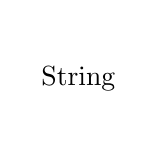
\begin{tikzpicture}[ 
	label distance=3mm,
	every label/.style={blue},
	event/.style={rectangle, draw, text centered,anchor=north},
	edge from parent/.style={very thick,draw=black!70,-latex},
	edge from parent path={(\tikzparentnode.south) -- ++(0,-0.50cm)-| (\tikzchildnode.north)},
	]
	\node [circle] (){String}
	
	;\end{tikzpicture}
	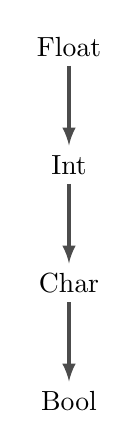
\begin{tikzpicture}
	[ 
	label distance=3mm,
	every label/.style={blue},
	event/.style={rectangle,draw,text centered,anchor=north},
	edge from parent/.style={very thick,draw=black!70,-latex},
	edge from parent path={(\tikzparentnode.south) -- ++(0,-0.50cm)-| (\tikzchildnode.north)},
	]
	\node []{Float}
	child {node {Int}
		child{ node {Char} 
			child { node {Bool}}
		}
	};
	\end{tikzpicture}
	\caption{Rappresentazione grafica della compatibilità tra tipi base.}
	\label{tab:albero}
\end{figure}


Oltre ai tipi di base  sono presenti due tipi composti: \texttt{*typ}, puntatore a \texttt{typ} e \texttt{Array[typ](dim)}, array di dimensione \texttt{dim} di elementi di tipo \texttt{typ}, dove \texttt{typ} è un tipo base o un tipo composto e \texttt{dim} è un intero; il tipo speciale \texttt{*Void} è utilizzato internamente per codificare il valore \texttt{Null}. È possibile assegnare il valore \texttt{Null} a qualsiasi elemento di tipo puntatore a \texttt{typ} qualunque sia il tipo \texttt{typ} puntato.
I tipi composti seguono le seguenti regole di compatibilità:
\begin{itemize}
\item un elemento di tipo \texttt{*typ1} è compatibile unicamente con elementi di tipo \texttt{*typ2}, un elemento di tipo \texttt{*typ1} è compatibile con un elemento di tipo \texttt{*typ2} se e solo se \texttt{typ1} è compatibile con \texttt{typ2} o se \texttt{typ1} = \texttt{Void};
\item un elemento di tipo \texttt{Array[typ1](dim1)} è compatibile unicamente con elementi di tipo \texttt{Array[typ2](dim2)}, un elemento di tipo \texttt{Array[typ1](dim1)} è compatibile con un elemento di tipo \texttt{Array[typ2](dim2)} se e solo \texttt{typ1} è compatibile con \texttt{typ2} e \texttt{dim1} = \texttt{dim2}.
\end{itemize}

Le regole di compatibilità tra tipi sono codificate all'interno della funzione \texttt{compatible} nel modulo \texttt{StaticAnalysis.hs}.
Sia \texttt{compatible typ1 typ2} equivalente a $typ_1 \leq typ_2$ nella notazione utilizzata in seguito, sia inoltre $\tau(exp)$ il tipo della espressione $exp$.
Le regole di derivazione per gli operatori unari sono riportare in tabella \ref{tab:unari}.

\begin{table}[]
\resizebox{\textwidth}{!}{
\begin{tabular}{l|l|l}
Operatore & Vincoli            & Tipo \\ \hline
$!exp$      & $\tau(exp) = Bool$ & $Bool$          \\
$-exp$      & $\tau(exp) \leq Float$   & \texttt{if} $\tau(exp) = Float$ \texttt{then} $Float$ \texttt{else} $Int$ \\
\end{tabular}
}
\caption{Regole di derivazione per gli operatori unari.}
\label{tab:unari}
\end{table}

Gli operatori binari sono classificati in \texttt{numerici}, \texttt{booleani}, \texttt{relazionali} come riportato in tabella \ref{tab:tipoOpBinari}. Le regole di derivazione per gli operatori binari sono definite in base alle possibili classi, tali regole sono riportate in tabella \ref{tab:binari}.

\begin{table}[]
\begin{tabular}{l|l}
Classe & Membri \\ \hline
Numerici & $\texttt{+},\ \texttt{-},\ \texttt{*},\ \texttt{/},\ \texttt{\^{}},\ \texttt{\%}$\\
Booleani & $\texttt{||},\ \texttt{\&\&}$ \\
Relazionali &$\texttt{<},\ \texttt{<=},\ \texttt{>},\ \texttt{>=} , \texttt{==},\ \texttt{!=} $ \\
\end{tabular}
\caption{Classificazione operatori binari.}
\label{tab:tipoOpBinari}
\end{table}

\begin{table}[]
\resizebox{\textwidth}{!}{
\begin{tabular}{l|l|l}
Operatore         &         Vincoli            & Tipo \\ \hline
$e_1\ op\ e_2$ t.c. $op \in Numerici$  &  $max(\tau(e_1), \tau(e_2)) \leq Float$ &  \texttt{if} $\tau(max(\tau(e_1), \tau(e_2))) = Float$ \texttt{then} $Float$ \texttt{else} $Int$ \\
$e_1\ op\ e_2$ t.c $op \in Booleani$ & $\tau(e_1) \leq Bool \wedge \tau(e_2) \leq Bool$ & $Bool$ \\
$e_1\ op\ e_2$ t.c. $op \in Relazionali$ & $\tau(e_1) \leq \tau(e_2) \wedge \tau(e_2) \leq \tau(e_1)$ & $Bool$\\
\end{tabular}
}
\caption{Regole di derivazione per gli operatori binari.}
\label{tab:binari}
\end{table}

Le regole di inferenza per le altre espressioni sono riportate in tabella \ref{tab:altro}.

\begin{table}[]
\resizebox{\textwidth}{!}{
\begin{tabular}{l|l|l}
Operatore         &         Vincoli            & Tipo \\ \hline
Array($e_1$, $\dots$, $e_n$) & $\forall_i (\tau(e_i) \leq max(\rbrace \tau(e_1), \dots, \tau(e_n)\rbrace)$ & $Array[max(\lbrace \tau(e_1), \dots, \tau(e_n)\rbrace)][n]$\\
if $e_c$ then $e_T$ else $e_F$ & $e_c \leq Bool \wedge e_T \leq max(\tau(e_T), \tau(e_F)) \wedge e_F \leq max(\tau(e_T), \tau(e_F))$ & $max(\tau(e_T), \tau(e_F)$\\
\end{tabular}
}

\caption{Regole di derivazione per l'operatore di creazione di array e l'operatore condizionale.}
\label{tab:altro}
\end{table}

Riguardo alle $L$-espressioni, ogni identificatore all'interno di un programma \texttt{Scala40} ha associato un tipo, nel caso delle variabili tale tipo è il tipo di dichiarazione della variabile, nel caso delle funzioni è il loro tipo di ritorno. Le regole di derivazione per gli operatori su $L$-espressioni di accesso ad un array, referenziamento e dereferenziamento sono riportate in tabella \ref{tab:LExp}.

\begin{table}[]
\resizebox{\textwidth}{!}{
\begin{tabular}{l|l|l}
Operatore         &         Vincoli            & Tipo \\ \hline
$*lexp$ & $\tau(lexp) = *typ$ dove $typ$ è un tipo qualsiasi & $typ$ \\
$\&lexp$ &                                                                                    & $*\tau(lexp)$\\
$lexp[e_a]$ & $\tau(e_a) \leq Bool \wedge \tau(lexp) = Array[typ](dim)$  con $typ$ e $dim$ qualsiasi & $typ$\\
\end{tabular}
}
\caption{Regole di derivazione per gli operatori su $L$-espressioni.}
\label{tab:LExp}
\end{table}

Negli statement di assegnamento è richiesto che il tipo della $R$-espressione sia compatibile con il tipo della $L$-espressione a cui si vuole assegnare.
Negli statement condizionali è richiesto che la condizione sia una espressione compatibile con il tipo $Bool$, se così non è viene lanciato un errore.

\subsection*{Vincoli riguardanti procedure e funzioni}
Alle procedure è assegnato come tipo di ritorno il tipo interno \texttt{Void}.
La signature della procedura principale di un programma \texttt{Scala40} è fissata a \texttt{main () : Void}, se si tenta di dichiarare una funzione/procedura con identificatore \texttt{main} e signature diversa da \texttt{main () : Void} viene riportato un errore.
Le chiamate di procedura non possono essere utilizzate come espressioni in quanto non hanno alcun valore di ritorno.

Riguardo al passaggio dei parametri attuali nelle chiamate di funzioni/procedure si richiede che il parametro attuale sia una $L$-espressione nel caso in cui il corrispondente parametro formale sia dichiarato con modalità per \texttt{riferimento}, per \texttt{risultato} o per \texttt{valore-risultato}. Nel caso in cui il parametro formale sia dichiarato con modalità per \texttt{valore} non ci sono vincoli sul corrispondente parametro attuale.
Si richiede una corrispondenza bi-univoca tra la firma di una chiamata di procedura/funzione e la corrispondente firma di procedura/funzione, ogni parametro attuale oltre a rispettare i vincoli sulla modalità deve avere tipo compatibile con il tipo del corrispondente parametro formale.

Negli statement \texttt{return exp} si richiede che il tipo della espressione \texttt{exp} sia compatibile con il tipo dello scope in cui l'istruzione è contenuta, se così non è un errore viene lanciato.

Non è permesso utilizzare statement \texttt{return exp} all'interno di procedure, sono chiaramente permessi gli statement \texttt{return} senza espressione di ritorno; vale il viceversa nel caso delle funzioni.

\subsection*{Altri vincoli forti}
Gli statement \texttt{break} e \texttt{continue} sono utilizzabili solamente all'interno di cicli indeterminati (\texttt{while} e \texttt{do ... while}), nel caso ne si rilevi un utilizzo inappropriato viene lanciato un errore.

All'interno di un ciclo \texttt{for} la variabile di iterazione è considerata come una implicita dichiarazione locale del corpo.
\subsection*{Vincoli deboli}
La violazione dei seguenti vincoli non impedisce il proseguimento alle successive fasi della compilazione, tuttavia viene visualizzato un messaggio di avviso in quanto si ritiene che il comportamento ottenuto possa non essere quello cercato.

\begin{itemize}
	\item All'interno del blocco di codice di una funzione, deve essere presente almeno una istruzione $\texttt{return exp}$, con $\tau(exp)$ compatibile con il tipo di ritorno della funzione per ogni possibile percorso di esecuzione del blocco (per ogni valutazione delle guardie delle istruzioni $\texttt{if}$).
	\item Il programma deve contenere la dichiarazione di una procedura con firma $\texttt{main ()}$ al top level.
	\item Se una funzione viene chiamata senza assegnarne il valore di ritorno ad un'espressione.
\end{itemize}